\documentclass[bachelor, och, referat]{SCWorks}
% параметр - тип обучения - одно из значений:
%    spec     - специальность
%    bachelor - бакалавриат (по умолчанию)
%    master   - магистратура
% параметр - форма обучения - одно из значений:
%    och   - очное (по умолчанию)
%    zaoch - заочное
% параметр - тип работы - одно из значений:
%    referat    - реферат
%    coursework - курсовая работа (по умолчанию)
%    diploma    - дипломная работа
%    pract      - отчет по практике
% параметр - включение шрифта
%    times    - включение шрифта Times New Roman (если установлен)
%               по умолчанию выключен
\usepackage{subfigure}
\usepackage{tikz,pgfplots}
\pgfplotsset{compat=1.5}
\usepackage{float}

%\usepackage{titlesec}
\setcounter{secnumdepth}{4}
%\titleformat{\paragraph}
%{\normalfont\normalsize}{\theparagraph}{1em}{}
%\titlespacing*{\paragraph}
%{35.5pt}{3.25ex plus 1ex minus .2ex}{1.5ex plus .2ex}

\titleformat{\paragraph}[block]
{\hspace{1.25cm}\normalfont}
{\theparagraph}{1ex}{}
\titlespacing{\paragraph}
{0cm}{2ex plus 1ex minus .2ex}{.4ex plus.2ex}

% --------------------------------------------------------------------------%
\usepackage[T2A]{fontenc}
\usepackage[utf8]{inputenc}
\usepackage{graphicx}
\graphicspath{ {./img/} }
\usepackage{tempora}

\usepackage[sort,compress]{cite}
\usepackage{amsmath}
\usepackage{amssymb}
\usepackage{amsthm}
\usepackage{fancyvrb}
\usepackage{listings}
\usepackage{listingsutf8}
\usepackage{longtable}
\usepackage{array}
\usepackage[english,russian]{babel}

\usepackage[colorlinks=true, linkcolor=black]{hyperref}
\usepackage{url}

\usepackage{underscore}
\usepackage{setspace}
\usepackage{indentfirst} 
\usepackage{mathtools}
\usepackage{amsfonts}
\usepackage{enumitem}
\usepackage{tikz}

\usepackage{minted}
\setminted[python3]{style=bw, linenos, breaklines=true, fontsize=\footnotesize}

\newcommand{\eqdef}{\stackrel {\rm def}{=}}
\newcommand{\specialcell}[2][c]{%
\begin{tabular}[#1]{@{}c@{}}#2\end{tabular}}

\renewcommand\theFancyVerbLine{\small\arabic{FancyVerbLine}}

\newtheorem{lem}{Лемма}

\begin{document}

% Кафедра (в родительном падеже)
\chair{теоретических основ компьютерной безопасности и криптографии}

% Тема работы
\title{Нейронные сети. Обучение без учителя и кластеризация данных}

% Курс
\course{5}

% Группа
\group{531}

% Факультет (в родительном падеже) (по умолчанию "факультета КНиИТ")
\department{факультета КНиИТ}

% Специальность/направление код - наименование
%\napravlenie{09.03.04 "--- Программная инженерия}
%\napravlenie{010500 "--- Математическое обеспечение и администрирование информационных систем}
%\napravlenie{230100 "--- Информатика и вычислительная техника}
%\napravlenie{231000 "--- Программная инженерия}
\napravlenie{10.05.01 "--- Компьютерная безопасность}

% Для студентки. Для работы студента следующая команда не нужна.
% \studenttitle{Студентки}

% Фамилия, имя, отчество в родительном падеже
\author{Стаина Романа Игоревича}

% Заведующий кафедрой
\chtitle{} % степень, звание
\chname{}

%Научный руководитель (для реферата преподаватель проверяющий работу)
\satitle{доцент} %должность, степень, звание
\saname{И.~И.~Слеповичев}

% Руководитель практики от организации (только для практики,
% для остальных типов работ не используется)
% \patitle{к.ф.-м.н.}
% \paname{С.~В.~Миронов}

% Семестр (только для практики, для остальных
% типов работ не используется)
%\term{8}

% Наименование практики (только для практики, для остальных
% типов работ не используется)
%\practtype{преддипломная}

% Продолжительность практики (количество недель) (только для практики,
% для остальных типов работ не используется)
%\duration{4}

% Даты начала и окончания практики (только для практики, для остальных
% типов работ не используется)
%\practStart{30.04.2019}
%\practFinish{27.05.2019}

% Год выполнения отчета
\date{2023}

\maketitle

% Включение нумерации рисунков, формул и таблиц по разделам
% (по умолчанию - нумерация сквозная)
% (допускается оба вида нумерации)
% \secNumbering

%-------------------------------------------------------------------------------------------

% \begin{minted}[fontsize=\small]{MySQL}
% \end{minted}

% \begin{figure}[H]
%     \centering
%     \includegraphics[width=0.999\textwidth]{img/}
%     \caption{}
%     \label{easy_hack}
% \end{figure}

\tableofcontents

\intro 
Алгоритмы обучения с учителем нейронных сетей подразумевают наличие некоего внешнего звена, 
предоставляющего сети, кроме входных, также и целевые выходные образы. 
Для их успешного функционирования необходимо наличие экспертов, 
создающих на предварительном этапе для каждого входного образа эталонный выходной. 
Обучения без учителя, наоборот, не требует разметки данных. 
Система старается сама найти в них общие признаки и связи.

Нейронные сети, обученные без учителя, чаще всего используются
для задачи кластеризации данных, где выборка объектов разбивается на непересекающиеся подмножества, 
называемые кластерами, так, чтобы каждый кластер состоял из схожих объектов, 
а объекты разных кластеров существенно отличались. 

Кластеризация обычно применяется для следующих целей:
\begin{itemize}
    \item Визуализация данных (наглядное представление многомерных данных).
    \item Сегментация рынка (определение типов клиентов).
    \item Рекомендательные системы (на основе кластеризации пользователей можно предлагать им товары или услуги, которые могут их заинтересовать).
    \item Объединение близких точек на карте (может использоваться для сжатия изображений).
    \item Обнаружение выбросов (помогает выявить аномальные значения в наборе данных и устранить их).
\end{itemize}

\section{Кластеризация данных}
Формально задача кластеризации описывается следующим образом \cite{cluster}.
Дано множество объектов $I = \{ i_1, i_2, \dots, i_n \}$, 
каждый из которых характеризуется вектором $x_j, j = 1, \dots, n$
атрибутов (параметров): $x_j = \{ x_{j1}, \dots, x_{jm} \}$.
Требуется построить множество кластеров $C$ и отображение $F$
множества $I$ на множество $C$, то есть $F: I \rightarrow C$.
Задача кластеризации состоит в построении множества
\[ C = \{ c_1, c_2, \dots, c_k, \dots, c_g \}, \]
где $c_k$ -- кластер, содержащий <<похожие>> объекты из $I$:
\[ c_k = \{ i_j, i_p | i_j \in I, i_p \in I \text{ и } \rho(i_j, i_p) < \sigma \}, \; \; \; (5) \]
$\sigma$ -- величина, определяющая меру близости для включения объектов
в один кластер, $\rho(i_j, i_p)$ -- мера близости между объектами,
называемая расстоянием.

Если расстояние $\rho(i_j, i_p)$ меньше некоторого значения $\sigma$,
то объекты считаются близкими и помещаются в один кластер.
В противном случае считается, что объекты отличны друг от друга и их помещают в разные
кластеры. Условие $(5)$ известно как гипотеза компактности. 

Неотрицательное число $\rho(x, y)$ называется расстоянием (метрикой)
между векторами $x$ и $y$, если выполняются следующие условия: 
\begin{enumerate}
    \item $\rho(x, y) \geq 0$ для всех $x$ и $y$.
    \item $\rho(x, y) = 0$, тогда и только тогда, когда $x = y$.
    \item $\rho(x, y) = \rho(y, x)$.
    \item $\rho(x, y) \leq \rho(x, k) + \rho(k, y)$ -- неравенство треугольника.
\end{enumerate}

Евклидово расстояние между векторами $x$ и $y$ представляет собой 
евклидову норму разности векторов, или длину отрезка, соединяющего точки
$x$ и $y$. 

Евклидово расстояние является частным случаем расстояния
Минковского
\[ \rho_p(x, y) = (\sum_{i = 1}^{m}|x_i - y_i|^p)^{\frac{1}{p}} = ||x - y||_p, \]
где $||z||_p = \displaystyle(\sum_{i = 1}^{m}|z_i|^p)^{\frac{1}{p}}$ -- $p$-норма вектора $z$.
Тогда 2-норма — это евклидова норма. 

Другой частный случай -- 1-норма, которая называется манхэттенским
расстоянием (расстоянием городских кварталов)
\[ \rho_1(x, y) = \sum_{i = 1}^{m} |x_i - y_i| \]

Манхеттенское расстояние -- это расстояние, которое проходится,
двигаясь параллельно осям координат, как в Манхеттнене или других
городах с прямоугольной продольно-поперечной планировкой улиц. 

\subsection{Сигнальный метод обучения Хебба}
Сигнальный метод обучения Хебба заключается в изменении весов по следующему
правилу \cite{hebb1}:
\[ w_{ij}(t) = w_{ij}(t - 1) + \alpha \cdot y_i^{(n - 1)} \cdot y_j^{(n)} \; \; \; (1)\]
где $y_i^{(n - 1)}$ -- выходное значение нейрона $i$ слоя 
$(n - 1)$, $y_j^{(n)}$ -- выходное значение нейрона $j$ слоя $n$;
$w_{ij}(t)$ и $w_{ij}(t - 1)$ -- весовой коэффициент синапса, 
соединяющего эти нейроны, на итерациях $t$ и $t - 1$ соответственно,
$\alpha$ -- коэффициент скорости обучения. Здесь и далее, для
общности, под $n$ подразумевается произвольный слой сети. 
При обучении по данному методу усиливаются связи между возбужденными нейронами. 

Существует также и дифференциальный метод обучения Хебба.
\[ w_{ij}(t) = w_{ij}(t - 1) + \alpha \cdot [y_i^{(n-1)}(t) - 
y_i^{(n - 1)}(t - 1)] \cdot [y_j^{(n)}(t) - y_j^{(n)}(t - 1)] \; \; \; (2)\]
Здесь $y_i^{(n-1)}(t)$ и $y_i^{(n - 1)}(t - 1)$ -- выходное
значение нейрона $i$ слоя $n - 1$ соответственно на итерациях
$t$ и $t - 1$; $y_j^{(n)}(t)$ и $y_j^{(n)}(t - 1)$ -- то же самое
для нейрона $j$ слоя $n$. Как видно из формулы $(2)$,
сильнее всего обучаются синапсы, соединяющие те нейроны,
выходы которых наиболее динамично изменились в сторону увеличения.

Алгоритм Хебба основан на принципе ассоциативной памяти и позволяет нейронной сети устанавливать связи между входными и выходными данными \cite{hebb2}.
\begin{enumerate}
    \item На стадии инициализации всем весовым коэффициентам присваиваются небольшие
    случайные значения.
    \item На входы сети подается входной образ, и сигналы возбуждения распространяются по
    всем слоям согласно принципам классических прямопоточных сетей, 
    то есть для каждого нейрона рассчитывается взвешенная сумма его входов, 
    к которой затем применяется функция активации нейрона, в результате
    чего получается выходное значение $y_i^{(n)}, i = 0, \dots, M_i - 1$,
    где $M_i$ -- число нейронов в слое $i; n = 0, \dots, N - 1$, а $N$
    -- число слоёв в сети.
    \item На основании полученных выходных значений нейронов по формуле $(1)$ или $(2)$
    производится изменение весовых коэффициентов. 
    \item Цикл с шага 2, пока выходные значения сети не застабилизируются с заданной точностью.
\end{enumerate}

Применение этого способа определения завершения обучения, отличного от
использовавшегося для сети обратного распространения, обусловлено тем, что подстраиваемые
значения синапсов фактически не ограничены. 

На втором шаге цикла попеременно предъявляются все образы из входного набора.
Следует отметить, что вид откликов на каждый класс входных образов не известен
заранее и будет представлять собой произвольное сочетание состояний нейронов выходного
слоя, обусловленное случайным распределением весов на стадии инициализации. Вместе с тем,
сеть способна обобщать схожие образы, относя их к одному классу. Тестирование обученной
сети позволяет определить топологию классов в выходном слое. Для приведения откликов
обученной сети к удобному представлению можно дополнить сеть одним слоем, который,
например, по алгоритму обучения однослойного перцептрона необходимо заставить отображать
выходные реакции сети в требуемые образы.

\subsection{Сеть Кохонена}
Сети (слои) Кохонена относятся к самоорганизующимся нейронным сетям. 
Самоорганизующаяся сеть позволяет выявлять кластеры (группы) входных векторов, обладающих
некоторыми общими свойствами. Такая сеть состоит из нейронов типа WTA --
Winner Takes All -- победитель получает всё.

\begin{figure}[H]
    \centering
    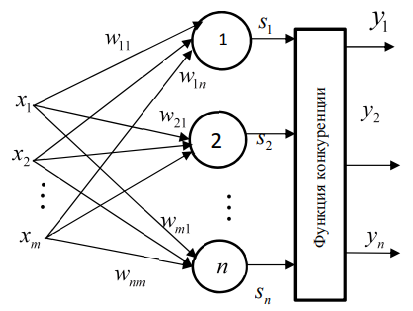
\includegraphics[width=0.6\textwidth]{6.png}
    \caption{Структура сети Кохонена}
\end{figure}

Каждый нейрон соединён со всеми компонентами $m$-мерного входного
векторак $x_i = (x_{i1}, \dots, x_{im})$.
Входной вектор -- это описание одного из
объектов, подлежащих кластеризации. Количество нейронов совпадает с
количеством кластеров, которое должна выделить сеть. В качестве нейронов
сети Кохонена применяются линейные взвешенные сумматоры 
\[ s_j = b_j + \sum_{i = 1}^{m} w_{ij} x_j, \]
где $j$ -- номер нейрона, $i$ -- номер входа, $s_j$ -- выход адаптивного сумматора,
$w_{ij}$ -- вес $i$-го входа $j$-го нейрона, $b_j$ -- порог.

Каждый $j$-ый нейрон описывается вектором весов $w_j = (w_{1j}, \dots, w_{mj})$, где
$m$ -- число компонентов входных векторов. С выходов адаптивных
сумматоров сигнал поступает на функцию конкуренции, работающую по
правилу <<победитель получает всё>>. Функция конкуренции находит выход
адаптивный сумматор с максимальным значением выхода. Пусть $k$ -- номер такого сумматора.
Тогда на выходе сети формируется выходной сигнал $y_k = 1$, остальные
выходные сигналы равны нулю. Если максимум
достигается одновременно на выходах нескольких сумматоров, то выходной
сигнал, равный единице, соответствует одному из них, например, первому. 

Обучение сети Кохонена представляет собой подбор значений весов,
минимизирующих ошибки от замены близких в смысле используемой
метрики входных векторов вектором весов. Такой подход называется
векторным квантованием и применяется в задачах сжатия аудио- и
видеосигналов. Идея векторного квантования состоит в компактном
представлении многомерных входных векторов с помощью ограниченного
набора опорных векторов меньшей размерности, образующих кодовую
таблицу. В случае сети Кохонена входные векторы кодируются номерами
нейронов-победителей (номерами кластеров). Таким образом, все векторы из
некоторой области входного пространства заменяются одним и тем же
опорным вектором, являющимся их ближайшим соседом. При использовании
евклидова расстояния входное пространство разбивается на многогранники
(мозаику) Вороного (Вороной Г. Ф.). Пример многогранников Вороного
для двумерного пространства приведен на рисунке \ref{voronoy}.

\begin{figure}[H]
    \centering
    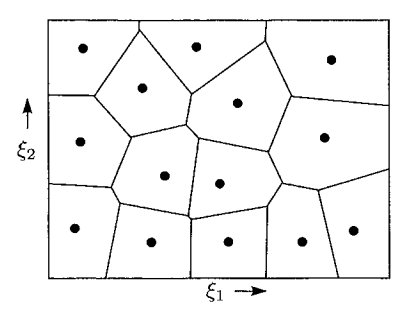
\includegraphics[width=0.5\textwidth]{7.png}
    \caption{Пример многогранников Вороного}
    \label{voronoy}
\end{figure}

В многомерном пространстве мозаика Вороного образуется
гиперплоскостями. 

\subsubsection{Обучение сети Кохонена}
Для обучения сети
применяются механизмы конкуренции. При подаче на вход сети вектора x
побеждает тот нейрон, вектор весов которого в наименьшей степени
отличаются от входного вектора. Для нейрона-победителя выполняется
соотношение
\[ \rho(x, w_j) = \min_{1 \leq i \leq n} \rho(x, w_i), \]
где $n$ -- количество нейронов, $j$ -- номер нейрона-победителя,
$\rho(x, w)$ -- расстояние между векторами $x$ и $w$.

Конкурирующая функция активации анализирует значения сумматоров и
формирует выходы нейронов, равные 0 для всех нейронов, кроме одного
<<нейрона-победителя>>, имеющего на выходе максимальное значение. Таким
образом, вектор выхода имеет единственный элемент, равный 1, который
соответствует нейрону-победителю, а остальные равны 0. Номер активного
нейрона определяет ту группу (кластер), к которой наиболее близок
входной вектор. 

В сети Кохонена входные значения желательно
нормировать. Для этого следует воспользоваться одной из следующих
формул: 
\[ x_{ni} = \frac{x_i}{\sqrt{\sum_{i=1}^{m} x_i^2}}, \; x_{ni} = \frac{x_i}{|x_i|} \]
Нормирование входных данных положительным образом сказывается на
скорости обучения сети.

Перед процессом обучения производится инициализация сети, то есть
первоначальное задание векторов весов. В простейшем случае задаются
случайные значения весов. Процесс обучения сети Кохонена состоит из
циклического повторения ряда шагов: 
\begin{enumerate}
    \item Подача исходных данных на входы. Обычно это случайная выборка
    одного из входных векторов.
    \item Нахождение выхода каждого нейрона. 
    \item Определение <<выигравшего>> нейрона (веса которого в наименьшей
    степени отличаются от соответствующих компонентов входного вектора),
    или нейрона-победителя. 
    \item Корректировка весов <<выигравшего>> нейрона по правилу Кохонена:
    \[ w_i^{(k + 1)} = w_i^{(k)} + \alpha_i^{(k)} [x - w_i^{(k)}], \; \; \; (3) \]
    где $x$ -- входной вектор, $k$ -- номер цикла обучения, 
    $\alpha_i^{(k)}$ -- коэффициент скорости обучения $i$-го нейрона 
    в $k$-ом цикле обучен6ия.
    \item Переход на шаг 1, если обучение не завершено.
\end{enumerate}

Таким образом, нейрон, чей вектор весов был ближе к входному вектору,
обновляется, чтобы быть еще ближе. В результате этот нейрон, скорее всего,
выиграет конкуренцию при подаче на вход близкого вектора и проиграет
при подаче существенно отличающегося вектора. После многократной
подачи обучающих векторов будет иметься нейрон, который выдает 1, когда
вектор принадлежит кластеру, и 0, когда вектор не принадлежит кластеру.
Таким образом, сеть учится классифицировать входные векторы. 

При обучении сети Кохонена возникает проблема так называемых
<<мертвых>> нейронов. Одно из ограничений всякого конкурирующего слоя
состоит в том, что некоторые нейроны оказываются незадействованными.
Это проявляется в том, что нейроны, имеющие начальные весовые векторы,
значительно удаленные от векторов входа, никогда не выигрывают
конкуренции, независимо от того, как долго продолжается обучение. В
результате оказывается, что такие векторы не используются при обучении и
соответствующие нейроны никогда не оказываются победителями. Такие
<<нейроны-неудачники>> называют <<мертвыми>> нейронами, поскольку они не
выполняют никакой полезной функции. Таким образом, входные данные
будут интерпретироваться меньшим числом нейронов. Поэтому надо дать
шанс победить всем нейронам. Для этого алгоритм обучения модифицируют
таким образом, чтобы <<мертвые>> нейроны участвовали в обучении. 

Например, алгоритм обучения модифицируют таким образом, чтобы
\\нейрон-победитель терял активность. Одним из приемов учета активности
нейронов является подсчет потенциала $p_i$ каждого нейрона в процессе
обучения. Первоначально нейронам присваивается потенциал
$p_i(0) = \frac{1}{n}$, где $n$ -- число нейронов. В $k$-ом цикле обучения
потенциал определяется по правилам:
\begin{equation*}
    p_i(k) = 
    \begin{cases}
        p_i(k - 1) + \frac{1}{n},  & \text{если } i \neq j,\\
        p_i(k - 1) - p_{min},  & \text{если } i = j,
    \end{cases}
\end{equation*}
где $j$ -- номер нейрона-победителя.

Если значение потенциала $p_i(k)$ падает ниже уровня $p_{min}$, то нейрон
исключается из рассмотрения -- <<отдыхает>>. При $p_{min} = 0$ нейроны не
исключаются из борьбы. При $p_{min} = 1$ нейроны побеждают по очереди, так
как в каждый цикл обучения только один из них готов к борьбе. На практике
хороший результат получается при $p_{min} \approx 0.75$.

На основе рассмотренного выше метода обучения сети строятся нейронные сети особого типа -- так
называемые самоорганизующиеся структуры -- self-organizing maps. 
\subsection{Карты Кохонена}
Карты Кохонена (самоорганизующиеся карты, или SOM —
self-organizing map)  предназначены для визуального представления
многомерных свойств объектов на двумерной карте. Карты Кохонена
производят отображение входных данных высокой размерности на элементы
регулярного массива малой размерности (обычно, двумерного). Карты
Кохонена похожи на сети Кохонена. Отличие состоит в том, что в карте
нейроны, являющиеся центрами кластеров, упорядочены в некоторую
структуру (обычно двумерную сетку). В процессе обучения карты
настраиваются веса не только нейрона-победитель, но и его соседей. В
результате близкие по некоторой метрике входные векторы в сети Кохонена
относятся к одному нейрону (центру кластера), а в карте Кохонена могут
относиться к разным близко расположенным на сетке нейронам. Обычно
нейроны располагаются в узлах двумерной сетки с прямоугольными или
шестиугольными ячейками. Нейроны-соседи определяются расстоянием
между нейронами на карте. На рисунке \ref{map} показаны шестиугольные и
прямоугольные ячейки, в центрах которых располагаются нейроны.
Шестиугольные ячейки более корректно отображают декартово расстояние
между объектами на карте, т. к. для этих ячеек расстояние между центрами
смежных ячеек одинаковы. 

\begin{figure}[H]
    \centering
    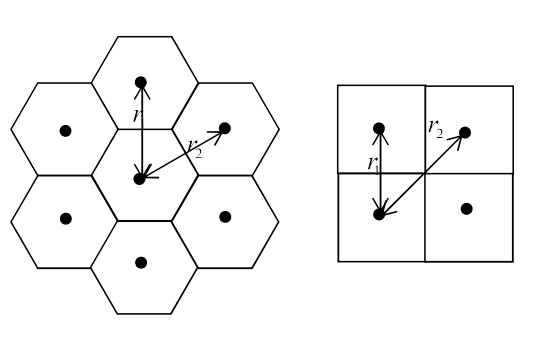
\includegraphics[width=0.5\textwidth]{8.png}
    \caption{Шестиугольные и прямоугольные ячейки}
    \label{map}
\end{figure}

Каждой ячейке соответствует нейрон сети Кохонена. То есть в карте
Кохонена число нейронов равно числу ячеек карты и больше числа нейронов
сети Кохонена, равного числу кластеров. Число ячеек карты зависит от
требуемой детальности изображения и подбирается экспериментально. 

Для каждой ячейки вычисляется одна из статистических характеристик
выбранного компонента входных векторов, попавших в ячейку. В
зависимости от величины этой характеристики ячейка окрашивается в
определенный цвет

Карты Кохонена только позволяют по раскраске ячеек карты выдвигать
гипотезы о наличии кластерной структуры и числе кластеров, зависимостях
между значениями отдельных переменных. Выдвинутые гипотезы должны
проверяться и подтверждаться иными способами. Карты используются на
стадии разведочного анализа данных, скорее для общего понимания задачи,
чем для получения каких-либо точных результатов. 

Существует несколько методов обучения карт Кохонена:
\begin{enumerate}
    \item Алгоритм последовательного обучения. Обновление весов
    производится после каждого обучающего примера. Обучение нейронов
    производится аналогично обучению нейронов сети Кохонена. Отличие
    состоит в том, что кроме нейрона-победителя обучаются нейроны, входящие
    в окрестность, или радиус обучения нейрона-победителя.
    Нейрон принадлежит окрестности нейрона-победителя,
    если расстояние между ним и нейроном-победителем на карте меньше
    определенной величины (в процессе обучения изменяются веса нейронов, но
    их положение на карте не изменяется). Такой алгоритм называют алгоритмом
    типа WTM (Winner Takes Most — победитель получает больше). В
    классическом алгоритме веса нейрона-победителя и всех нейронов, лежащих
    в пределах его окрестности, подвергаются обучению (адаптации) по
    несколько измененному правилу Кохонена. Веса нейронов, находящихся
    за пределами окрестности не изменяются. Размер окрестности и
    коэффициент скорости обучения являются функциями, значения которых
    уменьшаются с увеличением номера цикла обучения. 

    \item Алгоритм пакетного обучения. В этом алгоритме сначала предъявляются все
    примеры, а потом производится обновление весов.

    \item Алгоритм нейронного газа. Назван из-за подобия его
    динамики движению газа, обеспечивает большую скорость сходимости, чем
    рассмотренные алгоритмы. Алгоритм начинает с инициализации нейронов в пространстве данных. Затем он итеративно обновляет позиции нейронов в соответствии с близостью к данным. Нейроны, ближе всего к текущему образцу данных, перемещаются ближе к этому образцу, в то время как более далекие нейроны двигаются в меньшей степени.
    Таким образом, алгоритм нейронного газа позволяет нейронам "учиться" на основе структуры данных, и в результате формируется карта кластеров, которая отображает структуру данных. Этот метод может быть использован для кластеризации данных, снижения размерности и визуализации данных.
\end{enumerate}

\subsection{Метод k-средних}
Это наиболее популярный метод кластеризации. Цель алгоритма -- минимизировать сумму квадратов внутрикластерных расстояний до центра кластера \cite{kmean1}. Функция потерь (или целевая функция) имеет вид:
\[ J = \sum_{j = 1}^{k} \sum_{x \in C_i} (x - \mu_i)^2 , \]
где $k$ -- число кластеров, $C_i$ -- полученные кластеры, $\mu_i$ --
центры масс всех векторов $x$ из кластера $C_i$.

\subsubsection{Пример работы алгоритма}
Действие алгоритма в двумерном случае. Начальные точки выбраны случайно \cite{kmean2}.
\begin{figure}[H]
    \centering
    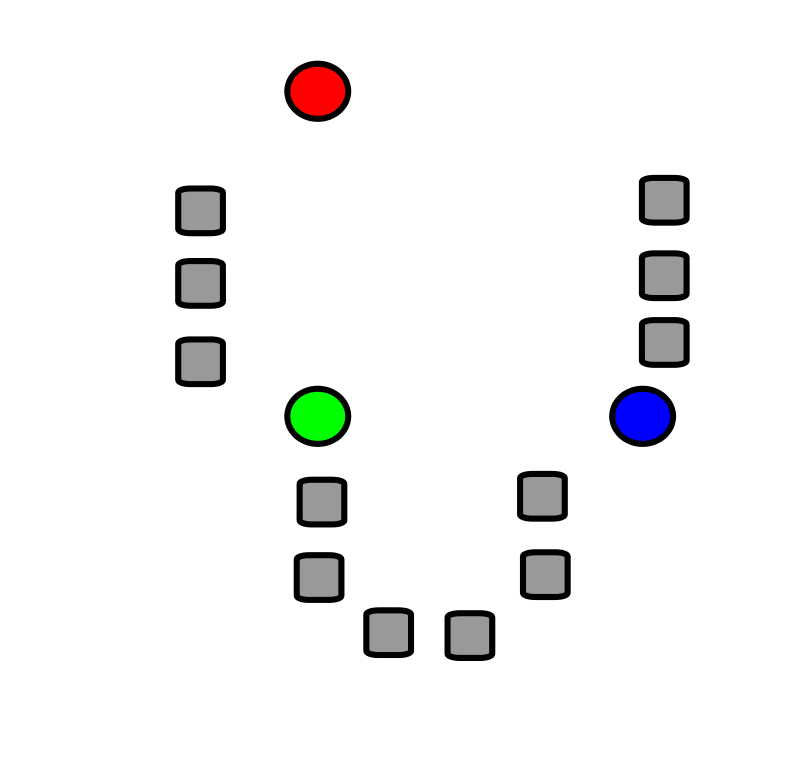
\includegraphics[width=0.5\textwidth]{1.png}
    \caption{Исходные точки и случайно выбранные начальные центры}
\end{figure}

\begin{figure}[H]
    \centering
    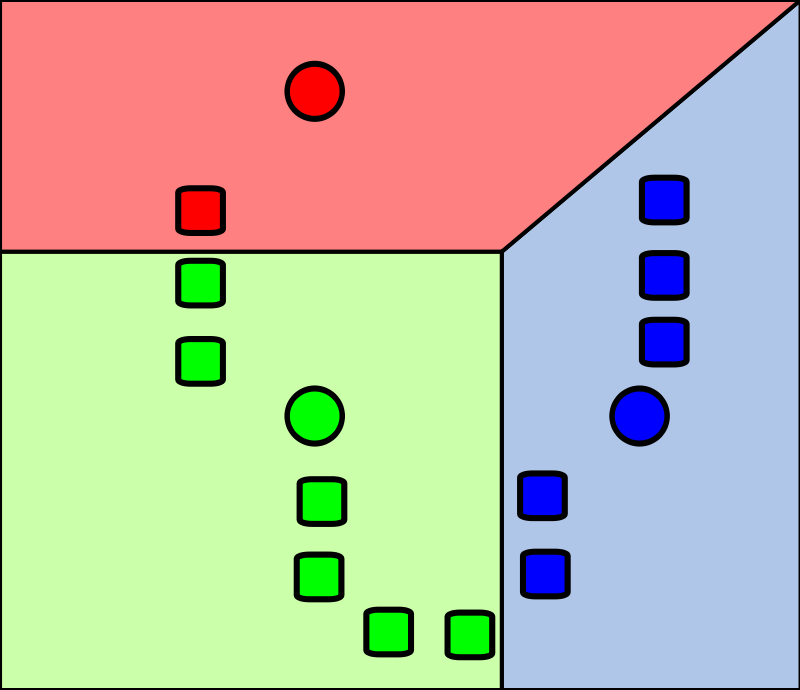
\includegraphics[width=0.5\textwidth]{2.png}
    \caption{Точки, отнесённые к начальным центрам}
\end{figure}

\begin{figure}[H]
    \centering
    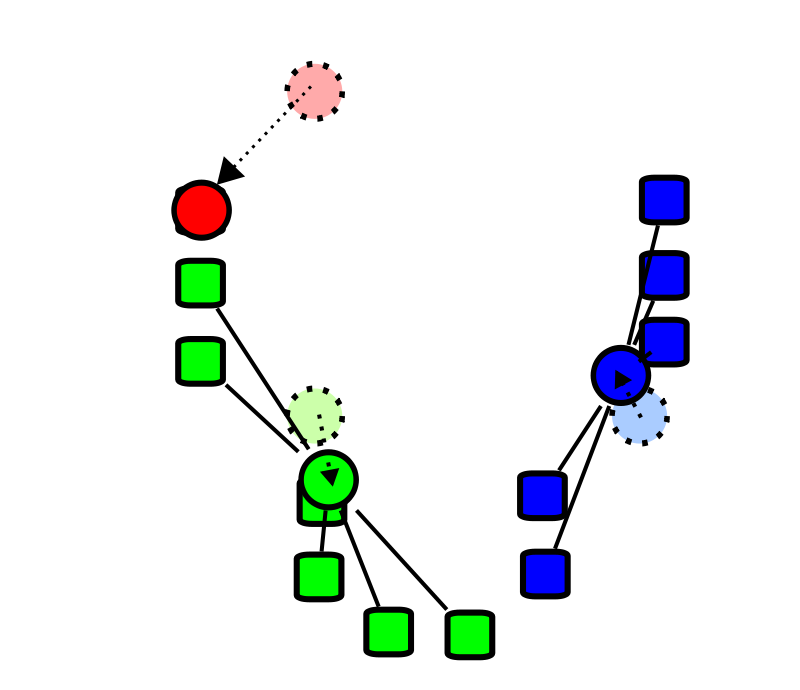
\includegraphics[width=0.5\textwidth]{3.png}
    \caption{Вычисление новых центров кластеров}
\end{figure}

\begin{figure}[H]
    \centering
    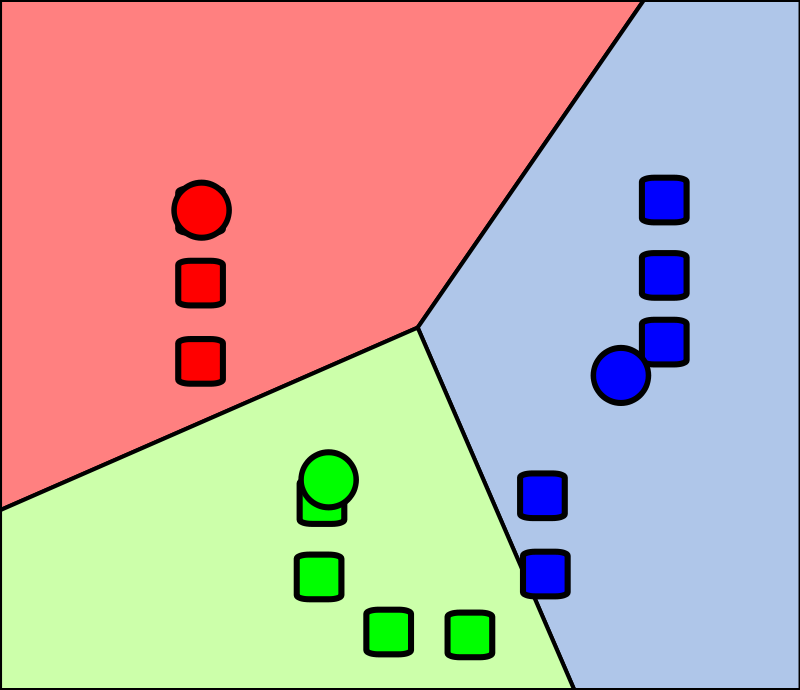
\includegraphics[width=0.5\textwidth]{4.png}
    \caption{Точки, отнесённые к новым центрам}
\end{figure}

Предыдущие шаги, за исключением первого, повторяются, пока алгоритм не сойдётся.

\subsubsection{Проблемы метода}
На вход алгоритма должно подаваться количество кластеров.
Есть два способа выбора количества кластеров:
\begin{enumerate}
    \item Экспертный метод (domain knowledge). Выбор количества кластеров будет зависеть от знания о предметной области.
    \item Метод локтя (elbow method). Можно обучить модель используя несколько вариантов количества кластеров, измерить сумму квадратов внутрикластерных расстояний и выбрать тот вариант, при котором данное расстояние перестанет существенно уменьшаться.
\end{enumerate}

Так же не гарантируется достижение глобального минимума суммарного квадратичного отклонения $J$, а только одного из локальных минимумов. И результат зависит от выбора исходных центров кластеров, их оптимальный выбор неизвестен.

\subsection{DBSCAN}
Основанная на плотности пространственная кластеризация для приложений с шумами (Density-based spatial clustering of applications with noise, \\DBSCAN) -- алгоритм кластеризации, основанной на плотности -- если дан набор точек в некотором пространстве, алгоритм группирует вместе точки, которые тесно расположены, помечая как выбросы точки, которые находятся одиноко в областях с малой плотностью (ближайшие соседи которых лежат далеко) \cite{dbscan}.

Рассмотрим набор точек в некотором пространстве, требующий кластеризации. Для выполнения кластеризации DBSCAN точки делятся на основные точки, достижимые по плотности точки и выпадающие следующим образом:
\begin{enumerate}
    \item Точка p является основной точкой, если по меньшей мере $m$ точек находятся на расстоянии, не превосходящем 
    $\epsilon$  ($\epsilon$ является максимальным радиусом соседства от $p$), до неё (включая саму точку $p$). Говорят, что эти точки достижимы прямо из $p$.

    \item Точка $q$ прямо достижима из $p$, если точка $q$ находится на расстоянии, не большем 
    $\epsilon$ , от точки $p$ и $p$ должна быть основной точкой.

    \item Точка $q$ достижима из $p$, если имеется путь $p_1 = 1, \dots, p_n = q$, где
    каждая точка $p_{i + 1}$ достижима прямо из $p_i$ 
    (все точки на пути должны быть основными, за исключением $q$).

    \item Все точки, не достижимые из основных точек, считаются выбросами.
\end{enumerate}

Теперь, если $p$ является основной точкой, то она формирует кластер вместе со всеми точками (основными или неосновными), достижимые из этой точки. Каждый кластер содержит по меньшей мере одну основную точку. Неосновные точки могут быть частью кластера, но они формируют его «край», поскольку не могут быть использованы для достижения других точек.

\begin{figure}[H]
    \centering
    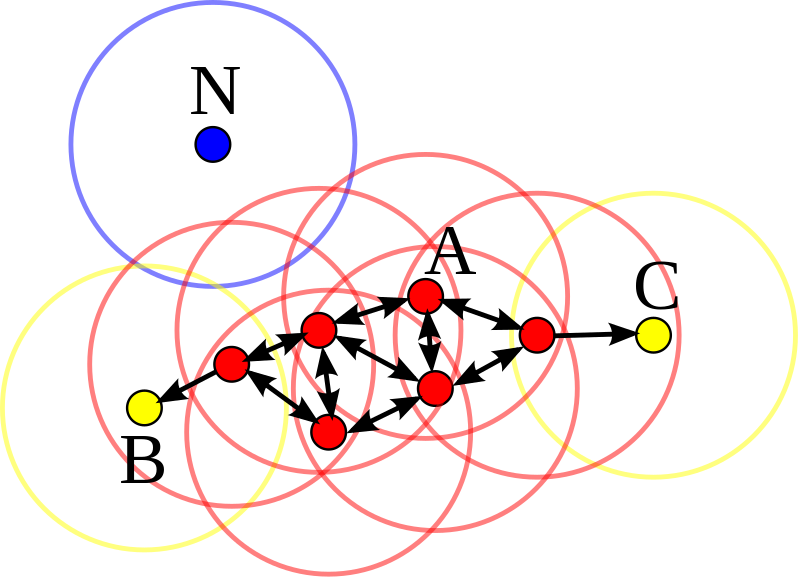
\includegraphics[width=0.5\textwidth]{5.png}
    \caption{Пример диаграммы с $m = 4$}
\end{figure}

Точка A и другие красные точки являются основными точками, поскольку область с радиусом 
$\epsilon$, окружающая эти точки, содержит по меньшей мере 4 точки (включая саму точку). Поскольку все они достижимы друг из друга, точки образуют один кластер. Точки $B$ и $C$ основными не являются, но достижимы из $A$ (через другие основные точки), и также принадлежат кластеру. Точка $N$ является точкой шума, она не является ни основной точкой, ни доступной прямо.

Достижимость не является симметричным отношением, поскольку, по определению, никакая точка не может быть достигнута из неосновной точки, независимо от расстояния (так что неосновная точка может быть достижимой, но ничто не может быть достигнуто из неё). Поэтому дальнейшее понятие связности необходимо для формального определения области кластеров, найденных алгоритмом DBSCAN. Две точки $p$ и $q$ связаны по плотности, если имеется точка $o$, такая что и $p$, и $q$ достижимы из o. Связность по плотности является симметричной.

Тогда кластер удовлетворяет двум свойствам:
\begin{enumerate}
    \item Все точки в кластере попарно связны по плотности.
    \item Если точка достижима по плотности из какой-то точки кластера, она также принадлежит кластеру.
\end{enumerate}

\subsubsection{Алгоритм}
DBSCAN требует задания двух параметров: 
$\epsilon$ и минимального числа точек, которые должны образовывать плотную область $m$. Алгоритм начинается с произвольной точки, которая ещё не просматривалась. Выбирается 
$\epsilon$-окрестность точки и, если она содержит достаточно много точек, образуется кластер, в противном случае точка помечается как шум. Заметим, что эта точка может быть позже найдена в 
$\epsilon$-окрестности другой точки и включена в какой-то кластер.

Если точка найдена как плотная точка кластера, её 
$\epsilon$-окрестность также является частью этого кластера. Следовательно, все точки, найденные в 
$\epsilon$-окрестности этой точки, добавляются к кластеру. Этот процесс продолжается, пока не будет найден связный по плотности кластер. Затем выбирается и обрабатывается новая непосещённая точка, что ведёт к обнаружению следующего кластера или шума.

DBSCAN может быть использован с любой функцией расстояния (а так же с функцией похожести или логическим условием). Функция расстояния может поэтому рассматриваться как дополнительный параметр.

\subsubsection{Преимущества и недостатки}
Преимущества:
\begin{enumerate}
    \item DBSCAN не требует спецификации числа кластеров в данных априори в отличие от метода k-средних.
    \item DBSCAN может найти кластеры произвольной формы. Он может найти даже кластеры полностью окружённые (но не связанные с) другими кластерами. Благодаря параметру MinPts уменьшается так называемый эффект одной связи (связь различных кластеров тонкой линией точек).
    \item DBSCAN имеет понятие шума и устойчив к выбросам.
    \item DBSCAN требует лишь двух параметров и большей частью нечувствителен к порядку точек в базе данных. (Однако, точки, находящиеся на границе двух различных кластеров могут оказаться в другом кластере, если изменить порядок точек, а назначение кластеров единственно с точностью до изоморфизма).
    \item DBSCAN разработан для применения с базами данных, которые позволяют ускорить запросы в диапазоне значений, например, с помощью R*-дерева.
    \item Параметры $m$ и $\epsilon$ могут быть установлены экспертами в рассматриваемой области, если данные хорошо понимаются.
\end{enumerate}

Недостатки:
\begin{enumerate}
    \item DBSCAN не полностью однозначен — краевые точки, которые могут быть достигнуты из более чем одного кластера, могут принадлежать любому из этих кластеров, что зависит от порядка просмотра точек. Для большинства наборов данных эти ситуации возникают редко и имеют малое влияние на результат кластеризации -- основные точки и шум DBSCAN обрабатывает однозначно. DBSCAN является вариантом, который трактует краевые точки как шум и тем самым достигается полностью однозначный результат, а также более согласованная статистическая интерпретация связных по плотности компонент.
    \item Качество DBSCAN зависит от измерения расстояния. Наиболее часто используемой метрикой расстояний является евклидова метрика. Особенно для кластеризации данных высокой размерности эта метрика может оказаться почти бесполезной ввиду так называемого «проклятия размерности», что делает трудным делом нахождение подходящего значения 
    $\epsilon$. Этот эффект, однако, присутствует в любом другом алгоритме, основанном на евклидовом расстоянии.

    \item DBSCAN не может хорошо кластеризовать наборы данных с большой разницей в плотности, поскольку не удается выбрать приемлемую для всех кластеров комбинацию $m - \epsilon$.
    \item Если данные и масштаб не вполне хорошо поняты, выбор осмысленного порога расстояния 
    $\epsilon$  может оказаться трудным.
\end{enumerate}

\conclusion
Таким образом, обучение без учителя -- это процесс обучения модели на основе неразмеченных данных, где нет известных меток или целевых переменных. В этом случае модель ищет скрытые структуры и закономерности в данных, чтобы создать представление или кластеризацию данных.

Преимуществами данного метода обучения являются:
\begin{enumerate}
    \item Извлечение скрытых структур. Обучение без учителя позволяет модели извлекать скрытые структуры и паттерны из данных, что может быть полезно для обнаружения новых знаний и понимания данных.
    \item Работа с большими объемами данных. Обучение без учителя может быть эффективным при работе с большими объемами данных, поскольку нет необходимости размечать каждый пример.
    \item Автоматическое обучение. Обучение без учителя позволяет модели самостоятельно находить паттерны и структуры в данных, без необходимости вручную определять правильные ответы.
\end{enumerate}

Недостатки:
\begin{enumerate}
    \item Неопределенность результатов. Результаты обучения без учителя могут быть менее интерпретируемыми и требуют дополнительного анализа и проверки.
    \item Трудность оценки. Оценка качества модели в обучении без учителя может быть сложной, поскольку нет явных правильных ответов для сравнения.
    \item Необходимость предварительной обработки данных. В обучении без учителя может потребоваться предварительная обработка данных для удаления шума или выбросов, что может быть трудоемким процессом.
\end{enumerate}

\begin{thebibliography}{10}
    \bibitem{hebb1}
    Короткий С. Нейронные сети: обучение без учителя [Электронный ресурс] -- URL: https://masters.donntu.ru/2006/kita/chvala/library/N3.pdf. (Дата обращения 11.01.2024). Загл. с экр. Яз. рус.

    \bibitem{hebb2}
    Обучение Хебба: простыми словами о принципах, алгоритме и применении в нейронных сетях [Электронный ресурс]. -- URL: https://skine.ru/articles/1511/
    (Дата обращения 11.01.2024). Загл. с экр. Яз. рус.

    \bibitem{cluster}
    Горбаченко В. И. Самоорганизация в нейронных сетях [Электронный ресурс] //Научно-исследовательский центр самоорганизации и развития систем.--2018. -- URL: http://gorbachenko.self-organization.ru/articles/Self-organizing_map.pdf. (Дата обращения 11.01.2024). Загл. с экр. Яз. рус.

    \bibitem{kmean1}
    Алгоритм кластеризации K-средних [Электронный ресурс]. -- URL: https://skine.ru/articles/1511/
    (Дата обращения 11.01.2024). Загл. с экр. Яз. рус.

    \bibitem{kmean2}
    Метод k-средних [Электронный ресурс]. -- URL: https://ru.wikipedia.org/wiki/Метод_k-средних
    (Дата обращения 11.01.2024). Загл. с экр. Яз. рус.

    \bibitem{dbscan}
    DBSCAN [Электронный ресурс]. -- URL: https://ru.wikipedia.org/wiki/DBSCAN
    (Дата обращения 11.01.2024). Загл. с экр. Яз. рус.
\end{thebibliography}

\end{document}